\documentclass[portrait,final,a0paper,fontscale=0.277]{baposter}

\usepackage{calc}
\usepackage{graphicx}
\usepackage{amsmath}
\usepackage{amssymb}
\usepackage{relsize}
\usepackage{multirow}
\usepackage{rotating}
\usepackage{bm}
\usepackage{url}
\usepackage{comment}
\usepackage{sidecap}

\usepackage{graphicx}
\usepackage{multicol}

%\usepackage{times}
%\usepackage{helvet}
%\usepackage{bookman}
\usepackage{palatino}

\newcommand{\captionfont}{\footnotesize}

\graphicspath{{images/}{../images/}}
\usetikzlibrary{calc}

\newcommand{\SET}[1]  {\ensuremath{\mathcal{#1}}}
\newcommand{\MAT}[1]  {\ensuremath{\boldsymbol{#1}}}
\newcommand{\VEC}[1]  {\ensuremath{\boldsymbol{#1}}}
\newcommand{\Video}{\SET{V}}
\newcommand{\video}{\VEC{f}}
\newcommand{\track}{x}
\newcommand{\Track}{\SET T}
\newcommand{\LMs}{\SET L}
\newcommand{\lm}{l}
\newcommand{\PosE}{\SET P}
\newcommand{\posE}{\VEC p}
\newcommand{\negE}{\VEC n}
\newcommand{\NegE}{\SET N}
\newcommand{\Occluded}{\SET O}
\newcommand{\occluded}{o}

%%%%%%%%%%%%%%%%%%%%%%%%%%%%%%%%%%%%%%%%%%%%%%%%%%%%%%%%%%%%%%%%%%%%%%%%%%%%%%%%
%%%% Some math symbols used in the text
%%%%%%%%%%%%%%%%%%%%%%%%%%%%%%%%%%%%%%%%%%%%%%%%%%%%%%%%%%%%%%%%%%%%%%%%%%%%%%%%

%%%%%%%%%%%%%%%%%%%%%%%%%%%%%%%%%%%%%%%%%%%%%%%%%%%%%%%%%%%%%%%%%%%%%%%%%%%%%%%%
% Multicol Settings
%%%%%%%%%%%%%%%%%%%%%%%%%%%%%%%%%%%%%%%%%%%%%%%%%%%%%%%%%%%%%%%%%%%%%%%%%%%%%%%%
\setlength{\columnsep}{1.5em}
\setlength{\columnseprule}{0mm}

%%%%%%%%%%%%%%%%%%%%%%%%%%%%%%%%%%%%%%%%%%%%%%%%%%%%%%%%%%%%%%%%%%%%%%%%%%%%%%%%
% Save space in lists. Use this after the opening of the list
%%%%%%%%%%%%%%%%%%%%%%%%%%%%%%%%%%%%%%%%%%%%%%%%%%%%%%%%%%%%%%%%%%%%%%%%%%%%%%%%
\newcommand{\compresslist}{%
\setlength{\itemsep}{1pt}%
\setlength{\parskip}{0pt}%
\setlength{\parsep}{0pt}%
}

%%%%%%%%%%%%%%%%%%%%%%%%%%%%%%%%%%%%%%%%%%%%%%%%%%%%%%%%%%%%%%%%%%%%%%%%%%%%%%
%%% Begin of Document
%%%%%%%%%%%%%%%%%%%%%%%%%%%%%%%%%%%%%%%%%%%%%%%%%%%%%%%%%%%%%%%%%%%%%%%%%%%%%%

\begin{document}

%%%%%%%%%%%%%%%%%%%%%%%%%%%%%%%%%%%%%%%%%%%%%%%%%%%%%%%%%%%%%%%%%%%%%%%%%%%%%%
%%% Here starts the poster
%%%---------------------------------------------------------------------------
%%% Format it to your taste with the options
%%%%%%%%%%%%%%%%%%%%%%%%%%%%%%%%%%%%%%%%%%%%%%%%%%%%%%%%%%%%%%%%%%%%%%%%%%%%%%
% Define some colors

%\definecolor{lightblue}{cmyk}{0.83,0.24,0,0.12}
\definecolor{lightblue}{rgb}{0.145,0.6666,1}
\definecolor{gold}{rgb}{0.545098,0.513725,0.470588}
\definecolor{silver}{rgb}{0.752941,0.752941,0.752941}
\definecolor{cyan}{rgb}{0,1,1}
\definecolor{backahead}{rgb}{1, 1,0.941176}
\definecolor{lefthead}{rgb}{0.941176, 1,0.941176}
\definecolor{righthead}{rgb}{0.933333,0.913725, 0.8}
\definecolor{backback}{rgb}{1,0.941176, 0.96078}
\definecolor{headfont}{rgb}{0.803922,0.5058824,0.3843137}


% Draw a video
\newlength{\FSZ}
\newcommand{\drawvideo}[3]{% [0 0.25 0.5 0.75 1 1.25 1.5]
   \noindent\pgfmathsetlength{\FSZ}{\linewidth/#2}
   \begin{tikzpicture}[outer sep=0pt,inner sep=0pt,x=\FSZ,y=\FSZ]
   \draw[color=lightblue!50!black] (0,0) node[outer sep=0pt,inner sep=0pt,text width=\linewidth,minimum height=0] (video) {\noindent#3};
   \path [fill=lightblue!50!black,line width=0pt] 
     (video.north west) rectangle ([yshift=\FSZ] video.north east) 
    \foreach \x in {1,2,...,#2} {
      {[rounded corners=0.6] ($(video.north west)+(-0.7,0.8)+(\x,0)$) rectangle +(0.4,-0.6)}
    }
;
   \path [fill=lightblue!50!black,line width=0pt] 
     ([yshift=-1\FSZ] video.south west) rectangle (video.south east) 
    \foreach \x in {1,2,...,#2} {
      {[rounded corners=0.6] ($(video.south west)+(-0.7,-0.2)+(\x,0)$) rectangle +(0.4,-0.6)}
    }
;
   \foreach \x in {1,...,#1} {
     \draw[color=lightblue!50!black] ([xshift=\x\linewidth/#1] video.north west) -- ([xshift=\x\linewidth/#1] video.south west);
   }
   \foreach \x in {0,#1} {
     \draw[color=lightblue!50!black] ([xshift=\x\linewidth/#1,yshift=1\FSZ] video.north west) -- ([xshift=\x\linewidth/#1,yshift=-1\FSZ] video.south west);
   }
   \end{tikzpicture}
}

\hyphenation{resolution occlusions}
%%
\begin{poster}%
  % Poster Options
  {
  % Show grid to help with alignment
  grid=false,
  % Column spacing
  colspacing=1em,
  % Color style
  bgColorOne=backback,
  bgColorTwo=lightblue,
  borderColor=gold,
  headerColorOne=lefthead,
  headerColorTwo=righthead,
  headerFontColor=headfont,
  boxColorOne=backahead,
  boxColorTwo=gold,
  % Format of textbox
  textborder=roundedleft,
  % Format of text header
  eyecatcher=true,
  headerborder=closed,
  headerheight=0.1\textheight,
%  textfont=\sc, An example of changing the text font
  headershape=roundedright,
  headershade=shadelr,
  headerfont=\Large\bf\textsc, %Sans Serif
  textfont={\setlength{\parindent}{1.5em}},
  boxshade=plain,
%  background=shade-tb,
  background=plain,
  linewidth=2pt
  }
    % University logo
  {% The makebox allows the title to flow into the logo, this is a hack because of the L shaped logo.
    
\includegraphics[height=8.0em]{images/logo}
  }
    % Title
  {\sf\bf {Non-Linear Dimensionality Reduction}\vspace{0.3 em}}
  % Authors
  {\smaller{YU.WU @liv.ac.uk}}
  % Eye Catcher
{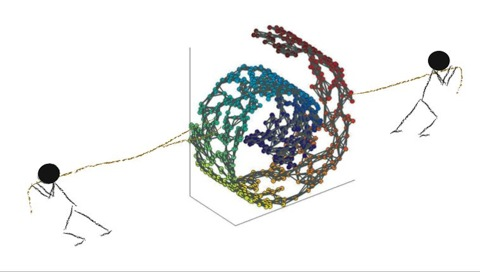
\includegraphics[height=6 em]{images/manifold}} 
  
  

%%%%%%%%%%%%%%%%%%%%%%%%%%%%%%%%%%%%%%%%%%%%%%%%%%%%%%%%%%%%%%%%%%%%%%%%%%%%%%
%%% Now define the boxes that make up the poster
%%%---------------------------------------------------------------------------
%%% Each box has a name and can be placed absolutely or relatively.
%%% The only inconvenience is that you can only specify a relative position 
%%% towards an already declared box. So if you have a box attached to the 
%%% bottom, one to the top and a third one which should be in between, you 
%%% have to specify the top and bottom boxes before you specify the middle 
%%% box.
%%%%%%%%%%%%%%%%%%%%%%%%%%%%%%%%%%%%%%%%%%%%%%%%%%%%%%%%%%%%%%%%%%%%%%%%%%%%%%
    %
    % A coloured circle useful as a bullet with an adjustably strong filling
    \newcommand{\colouredcircle}{%
      \tikz{\useasboundingbox (-0.2em,-0.32em) rectangle(0.2em,0.32em); \draw[draw=black,fill=lightblue,line width=0.03em] (0,0) circle(0.18em);}}

%%%%%%%%%%%%%%%%%%%%%%%%%%%%%%%%%%%%%%%%%%%%%%%%%%%%%%%%%%%%%%%%%%%%%%%%%%%%%%
  \headerbox{Abstract}{name=abstract,column=0,row=0}{
%%%%%%%%%%%%%%%%%%%%%%%%%%%%%%%%%%%%%%%%%%%%%%%%%%%%%%%%%%%%%%%%%%%%%%%%%%%%%%
   \begin{itemize}
   \item  Scientists working with large volumes of high-dimensional data, such as text/linguistic data, video/images, global climate patterns, stellar spectra, or human gene distributions, regularly confronted the problem to \emph{embed} data that originally lies in a high dimensional space in a lower dimensional space.
   \item  Because for any high dimensional data to be interesting, it must perceive some intrinsic low dimensional nature, which makes dimensionality reduction possible.
   \item  Laplacian Eigenmaps(LE)\cite{1} is therefore introduced as  one of the many Non-Linear Dimensionality Reduction( NLDR) techniques and various \emph{NLDR}  algorithms have been represented and compared.   
   \end{itemize}
      \vspace{-0.3em}
 }
 
  %%%%%%%%%%%%%%%%%%%%%%%%%%%%%%%%%%%%%%%%%%%%%%%%%%%%%%%%%%%%%%%%%%%%%%%%%%%%%%
  \headerbox{References}{name=references, span = 2, column=1,above=bottom}{
%%%%%%%%%%%%%%%%%%%%%%%%%%%%%%%%%%%%%%%%%%%%%%%%%%%%%%%%%%%%%%%%%%%%%%%%%%%%%%
    \smaller
    \bibliographystyle{ieee}
    \renewcommand{\section}[2]{\vskip 0.05em}
      \begin{thebibliography}{1}\itemsep=-0.01em
      \setlength{\baselineskip}{0.4em}
      \bibitem{1}
        Belkin, Mikhail and Niyogi, Partha.
        \newblock {L}aplacian {E}igenmaps for {D}imensionality {R}eduction and {D}ata {R}epresentation.
        \newblock In {\em Neural Computation}
      \bibitem{2}
        Van der Maaten, Laurens, and Geoffrey Hinton.
        \newblock {V}isualizing {D}ata {U}sing t-{SNE}.
        \newblock In {\em JMLR }
              \bibitem{3}
        Bordes, Antoine, et al.
        \newblock A {S}emantic {M}atching {E}nergy {F}unction for {L}earning {W}ith {M}ulti-relational {D}ata.
        \newblock In {\em Machine Learning }
      \end{thebibliography}
   \vspace{0.3em}
  }
%%%%%%%%%%%%%%%%%%%%%%%%%%%%%%%%%%%%%%%%%%%%%%%%%%%%%%%%%%%%%%%%%%%%%%%%%%%%%% 

%%%%%%%%%%%%%%%%%%%%%%%%%%%%%%%%%%%%%%%%%%%%%%%%%%%%%%%%%%%%%%%%%%%%%%%%%%%%%%
  \headerbox{Introduction}{name=introduction,column=0,below=abstract }{
%%%%%%%%%%%%%%%%%%%%%%%%%%%%%%%%%%%%%%%%%%%%%%%%%%%%%%%%%%%%%%%%%%%%%%%%%%%%%%
   A canonical problem in \emph{non-linear dimensional reduction} is illustrated in the following.
   
  % Isomap faces
  {% The makebox allows the title to flow into the logo
    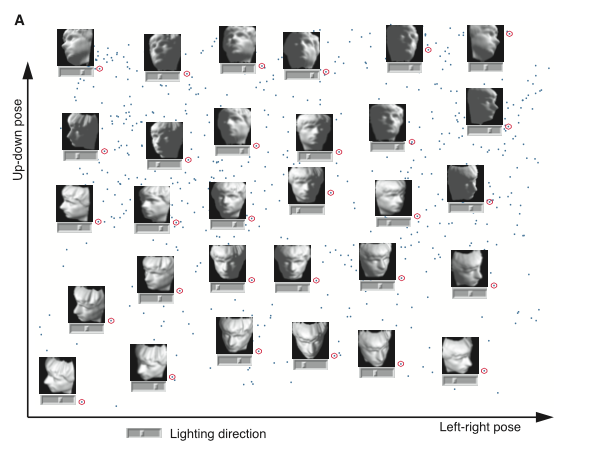
\includegraphics[width=0.92 \linewidth]{images/Isomap_faces}
    \indent \smaller{Embedding of High Dimensional Images}
  }
      \begin{enumerate}\compresslist
      \item  Many images of a person's face have been observed under different pose and lighting conditions, in no particular order.
      \item Although the input dimensionality may be quite high (e.g., 4096 for these 64 pixel by 64 pixel images), the perceptually meaningful structure of these images has many fewer independent degrees of freedom. 
      \item All  images lie on an intrinsically \emph{three-dimensional} manifold (see the above figure), or constraint surface, that can be parameterised by two pose variables plus an azimuthal lighting angle.       
     \end{enumerate}     
% \indent{ } Our goal is to discover, given only the unordered high-dimensional inputs, low-dimensional representations such as the above figure with coordinates that capture the intrinsic degrees of freedom of a data set. 
   \vspace{-0.3em}
  }

%%%%%%%%%%%%%%%%%%%%%%%%%%%%%%%%%%%%%%%%%%%%%%%%%%%%%%%%%%%%%%%%%%%%%%%%%%%%%%
  \headerbox{Methods}{name= methods,column=0,below=introduction, above = bottom }{
%%%%%%%%%%%%%%%%%%%%%%%%%%%%%%%%%%%%%%%%%%%%%%%%%%%%%%%%%%%%%%%%%%%%%%%%%%%%%%
\begin{multicols}{2}
   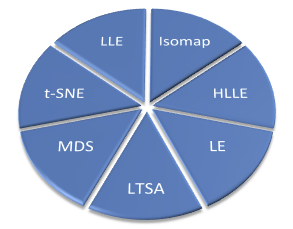
\includegraphics[width=0.65 \linewidth]{images/pie}
  
   \indent \smaller
   In the following, seven NDR algorithms in this pie chart have been experimented on one digits datasets. Among these, we have studied  the formulation of  Laplacian Eigenmaps (also referred as Spectral Embedding) algorithms .
   \end{multicols}
   \vspace{0.3 em}
  }
  

%%%%%%%%%%%%%%%%%%%%%%%%%%%%%%%%%%%%%%%%%%%%%%%%%%%%%%%%%%%%%%%%%%%%%%%%%%%%%%
  \headerbox{ Laplacian Eigenmaps}{name=background model,column=1, span =2, row = 0}{
%%%%%%%%%%%%%%%%%%%%%%%%%%%%%%%%%%%%%%%%%%%%%%%%%%%%%%%%%%%%%%%%%%%%%%%%%%%%%%
\begin{multicols}{2}
\noindent{ % graph for LE
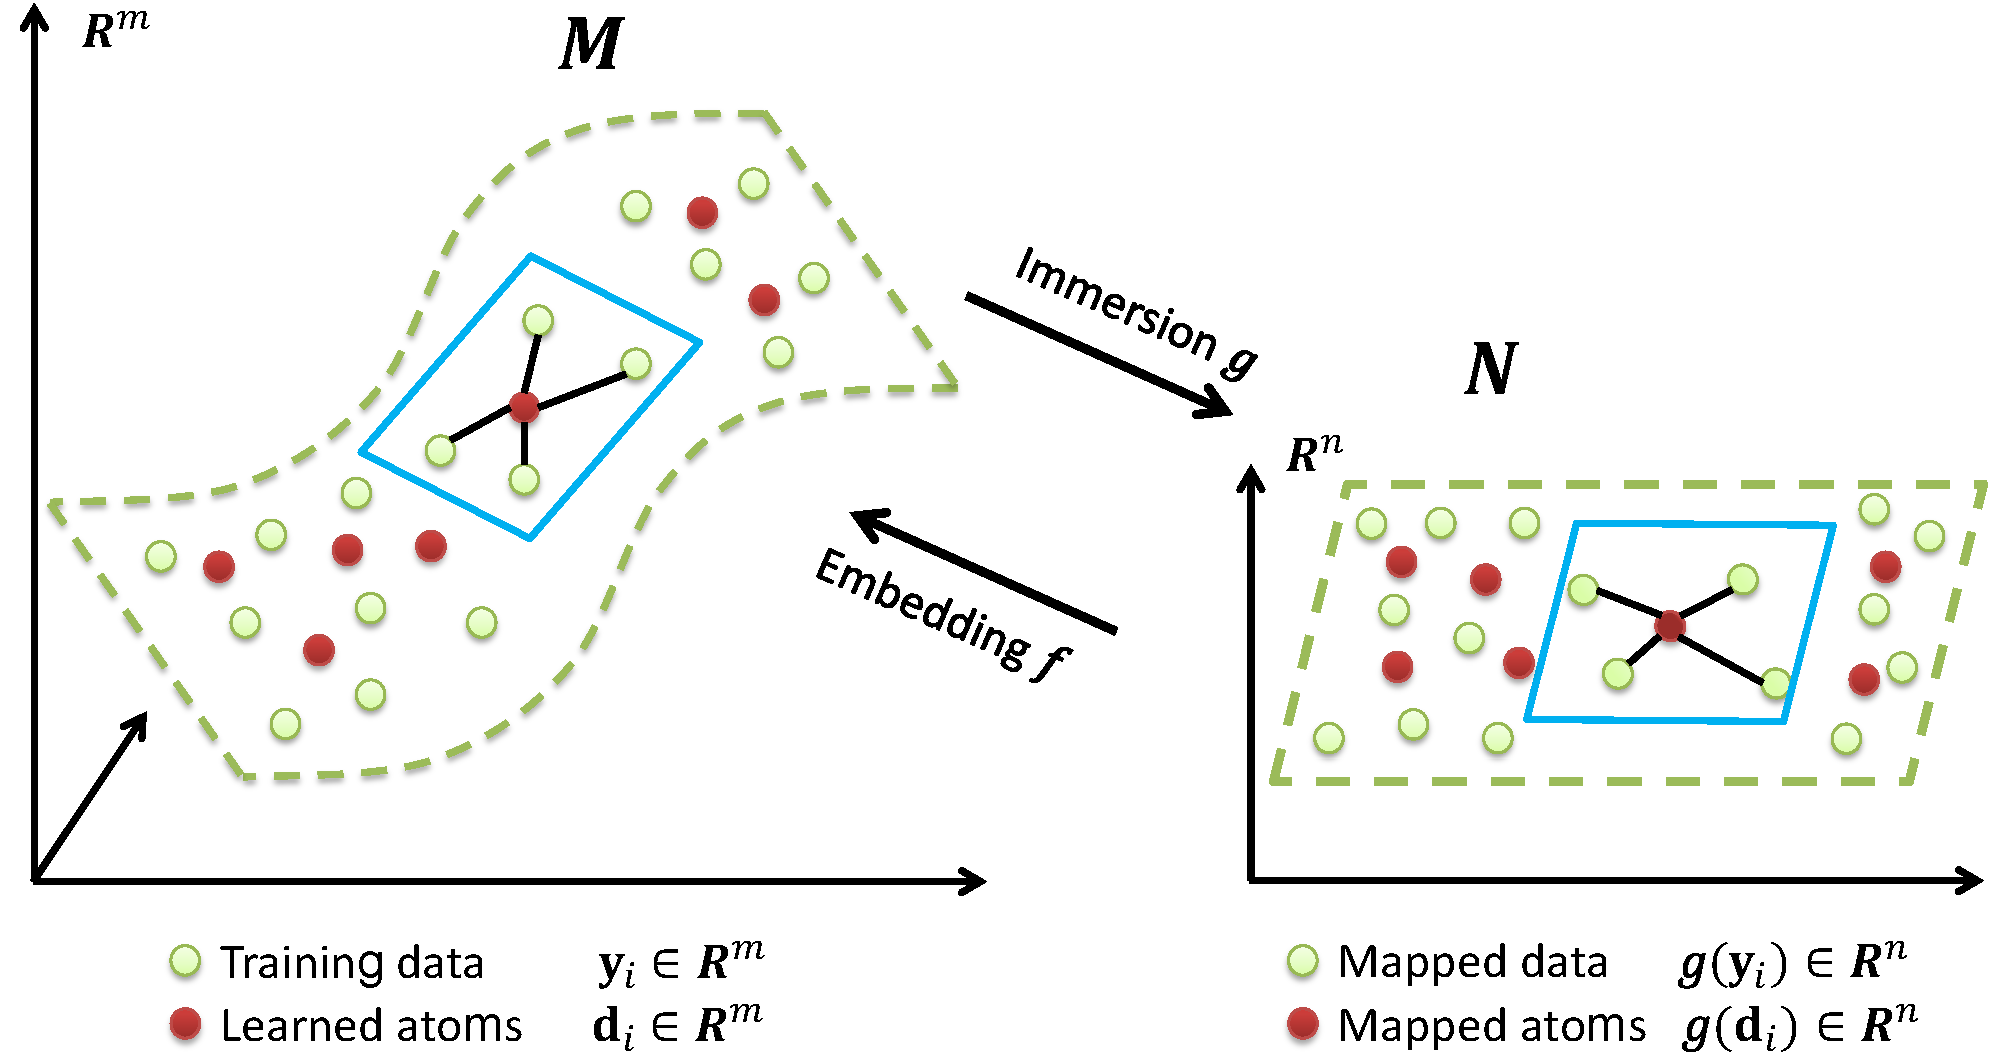
\includegraphics[width=0.92 \linewidth]{HighlowManifold.png} 
}

  \indent Considering the problem of representing all of the vectors in a set of $n$ $d$-dimensional samples $\bm{x}_1, \bm{x}_2, \ldots, \bm{x}_n$  by a single vector $\bm{y} = {y_1, y_2, \ldots, y_n}$ such that $y_i$ represents $\bm{x}_i$. 
  
 Laplacian Eigenmaps( also referred as Spectral Embedding) defines a ''good'' map by minimising the following objective functions under appropriate constraints,
 \begin{equation}
 \sum_{i,j}^n (y_i - y_j)^2 W_{ij}, \notag
 \end{equation}
 where matrix $\mathbf{W} = [W_{ij}]$ is a \emph{similarity matrix}. 
 
 This objective functions with the choice of symmetric weights $W_{ij}$( $W_{ij} = W_{ji}$) incurs a heavy penalty if neighbouring points $\bm{x}_i$ and $\bm{x}_j$ are mapped far apart, i.e, if $(y_i - y_j)^2$ is large. Therefore, minimising it is an attempt to ensure that, if $\bm{x}_i$ and $\bm{x}_j$ are ''close'', then $y_i$ and $y_j$ are close as well.
  \end{multicols}
   \vspace{0.3em}
  }
%%%%%%%%%%%%%%%%%%%%%%%%%%%%%%%%%%%%%%%%%%%%%%%%%%%%%%%%%%%%%%%%%%%%%%%%%%%%%%

%%%%%%%%%%%%%%%%%%%%%%%%%%%%%%%%%%%%%%%%%%%%%%%%%%%%%%%%%%%%%%%%%%%%%%%%%%%%%%
\headerbox{Results}{name=results,column=1,span=2, below = background model}{
  %%%%%%%%%%%%%%%%%%%%%%%%%%%%%%%%%%%%%%%%%%%%%%%%%%%%%%%%%%%%%%%%%%%%%%%%%%%%%%
\newcommand{\basiswidth}{0.35}
\newcommand{\basisskip}{-0.01} % (1-4*\basiswidth)/3
\newcommand{\imagegrid}[1]{
\begin{tabular}{@{}
  c@{\hspace{\basisskip\linewidth}}%
    c@{\hspace{\basisskip\linewidth}}%
  c@{\hspace{\basisskip\linewidth}}}
   %
\includegraphics[width=\basiswidth\linewidth,height=\basiswidth\linewidth,keepaspectratio]{#1-01} &
\includegraphics[width=\basiswidth\linewidth,height=\basiswidth\linewidth,keepaspectratio]{#1-02} &
\includegraphics[width=\basiswidth\linewidth,height=\basiswidth\linewidth,keepaspectratio]{#1-03} \vspace{-0.4em} \\
\includegraphics[width=\basiswidth\linewidth,height=\basiswidth\linewidth,keepaspectratio]{#1-04} &
\includegraphics[width=\basiswidth\linewidth,height=\basiswidth\linewidth,keepaspectratio]{#1-05} &
\includegraphics[width=\basiswidth\linewidth,height=\basiswidth\linewidth,keepaspectratio]{#1-06} \vspace{-0.4em} \\
\includegraphics[width=\basiswidth\linewidth,height=\basiswidth\linewidth,keepaspectratio]{#1-07} &
\includegraphics[width=\basiswidth\linewidth,height=\basiswidth\linewidth,keepaspectratio]{#1-08} & \\
\end{tabular}
}
\noindent\begin{tabular}{@{}c@{}}
\begin{minipage}{0.94\linewidth}
  \imagegrid{figure}
\end{minipage}\\
\smaller Comparison of Various NDR Algorithms Upon A  Selection of Digits Datasets
\end{tabular}\\[1em]

 %     \begin{multicols}{2}
%      \end{multicols}
      \vspace{-0.7em}
}
%%%%%%%%%%%%%%%%%%%%%%%%%%%%%%%%%%%%%%%%%%%%%%%%%%%%%%%%%%%%%%%%%%%%%%%%%%%%%%


  \headerbox{Source Code}{name=source,column=2,below=results,above=references}{
%%%%%%%%%%%%%%%%%%%%%%%%%%%%%%%%%%%%%%%%%%%%%%%%%%%%%%%%%%%%%%%%%%%%%%%%%%%%%%
  \noindent
  \begin{minipage}{\linewidth}
  \begin{minipage}{0.7\linewidth}
    \indent{}The source code for all algorithms are obtained at \\
  \end{minipage}\hfill%
  \begin{minipage}{0.28\linewidth}
  \hfill
\includegraphics[width=\linewidth]{chart}
  \end{minipage}
  \end{minipage}
  \url{http://scikit-learn.org/stable/modules/manifold.html}
  }
%%%%%%%%%%%%%%%%%%%%%%%%%%%%%%%%%%%%%%%%%%%%%%%%%%%%%%%%%%%%%%%%%%%%%%%%%%%%%%
  \headerbox{A Future Direction}{name=questions,column=1,span=1,below= results,above= references}{
%%%%%%%%%%%%%%%%%%%%%%%%%%%%%%%%%%%%%%%%%%%%%%%%%%%%%%%%%%%%%%%%%%%%%%%%%%%%%%
   NLDR algorithms also use pairwise \emph{similarity matrix} as input, thus, becomes potential  for developing relational learning algorithms\cite{1}\cite{2}, which aims at handling huge amounts of structured data generated daily in many application domains ranging from computational biology or information retrieval, to natural language processing.
    
       \vspace{0.3em}
  }
%%%%%%%%%%%%%%%%%%%%%%%%%%%%%%%%%%%%%%%%%%%%%%%%%%%%%%%%%%%%%%%%%%%%%%%%%%%%%%


\end{poster}

\end{document}

